%!TEX root = book.tex

\chapter{The Description of Radiation}
\label{chapter:description}

\noindent
In this chapter we'll consider how to describe radiation and also
consider the special characteristics of radiation in thermodynamic
equilibrium.

\newslide

\section{Different Perspectives on Radiation}

Depending on the properties we wish to emphasize and the level of
accuracy and approximation that we are willing to accept, we can
describe a radiation field in one of several ways:

\newslide

\begin{enumerate}

\item As a quantum-mechanical field. This is useful when we wish to
  consider the interaction of radiation with matter at the microscopic
  level -- the emission, absorption, or scattering of individual photons
  by individual atoms, molecules, or electrons. This description is the
  most accurate, but it is often not well suited to describing
  macroscopic phenomena.

\newslide

\item As a classical electromagnetic field. This description is familiar
  from undergraduate physics, but it is not especially useful in stellar
  atmospheres, as wave phenomena are only important for far-infrared and
  radio waves, which account for a negligible fraction of the total
  luminosity. Still, it is worth keeping in mind the possibility of wave
  phenomena when considering other applications of radiation transfer.

\newslide

\item As a semi-classical gas of photons. Again, this description is
  familiar from undergraduate physics. We consider the radiation to
  consist of a gas of photons traveling in straight lines at speed $c$
  and only being destroyed or created by discrete interactions with
  matter. This is useful as a bridge between the quantum mechanical and
  thermodynamic descriptions.

\newslide

\item As a flow of energy. This thermodynamic description is unlikely to
  be familiar from undergraduate physics, as undergraduate classical
  thermodynamics courses typically deal only with matter. However,
  considering radiation in this manner is extremely useful when
  considering the macroscopic thermodynamics of the atmosphere, such as
  the restriction that the atmosphere must be in thermal equilibrium.

\end{enumerate}

\newslide

We will use both the photon gas and energy flow descriptions in stellar
atmospheres. In reality, the two are closely linked, as photons carry
energy $h\nu$ at a speed $c$, so converting from one to the other often
involves little more than multiplication or division by factors of
$h\nu$ and $c$.

\newslide

\section{The Specific Intensity}

In radiation transfer we most commonly work with a somewhat unusual
macroscopic thermodynamic quantity called the specific intensity. The
reasons for this should soon become apparent.

\newslide

\subsection{Definition}

\begin{figure}
\begin{center}
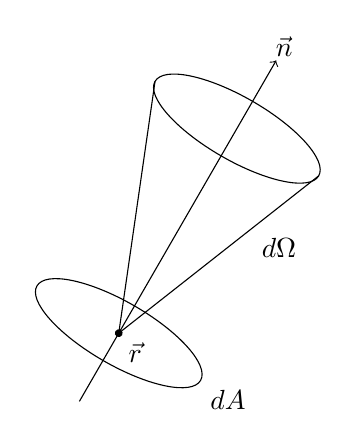
\begin{tikzpicture}
\begin{scope}[rotate=-30]
\fill[black] (0,0) circle [radius=0.05];
\draw[->] (0,-1) -- (0,4);
\draw(0,0) ellipse [x radius=1.2cm,y radius=0.4cm];
\draw(0,3) ellipse [x radius=1.2cm,y radius=0.4cm];
\draw(0,0) -- (-1.2,3);
\draw(0,0) -- (+1.2,3);
\draw (0,4.2) node {$\vec n$};
\draw (0,0) node[below right] {$\vec r$};
\draw (1.2,0) node[below right] {$dA$};
\draw (0.8,2) node[below right] {$d\Omega$};
\end{scope}
\end{tikzpicture}
\end{center}
\caption{The geometry used in the definition of the
specific intensity.}
\label{fig-specific-intensity-definition}
\end{figure}

Consider Figure \ref{fig-specific-intensity-definition}.
The specific intensity $I_\nu(\vec r, \vec n, \nu, t)$ at a
position $\vec r$, in a direction $\vec n$, at a frequency
$\nu$, and at a time $t$ is such that the energy $dE$
transported by radiation across an area $dA$, centered on
$\vec r$ and perpendicular to $\vec n$, into a solid angle
$d\Omega$ about $\vec n$, in a frequency interval $(\nu,
\nu+d\nu)$, in a time interval $(t,t+dt)$ is given by
\begin{align}
dE \equiv I_\nu(\vec r, \vec n, \nu, t)\,dA\,d\Omega\,d\nu\,dt.
\end{align}
The SI units of $I_\nu$ are
$\mathrm{W\,m^{-2}\,Hz^{-1}\,sr^{-1}}$ and the traditional units are $\mathrm{erg\,s^{-1}\,cm^{-2}\,Hz^{-1}\,sr^{-1}}$. The
specific intensity is sometimes called the brightness.

\newslide

Another form of the specific intensity is $I_\lambda$, the specific
intensity per unit wavelength instead of per unit frequency. The
definition of $I_\lambda$ is analogous to that of $I_\nu$, but $\lambda$
and $d\lambda$ replace $\nu$ and $d\nu$. That is,
\begin{align}
dE \equiv I_\lambda(\vec r, \vec n, \lambda, t)\,dA\,d\Omega\,d\lambda\,dt.
\end{align}
The SI units of
$I_\lambda$ are $\mathrm{W\,m^{-3}\,sr^{-1}}$ and the traditional units are $\mathrm{erg\,s^{-1}\,cm^{-2}\,\Angstrom^{-1}\,sr^{-1}}$
or sometimes $\mathrm{erg\,s^{-1}\,cm^{-2}\,\micron^{-1}\,sr^{-1}}$. Since the
energy $dE$ transferred is the same, regardless of whether we consider
$I_\nu$ or $I_\lambda$, we have
\begin{align}
I_\nu\,d\nu = I_\lambda\,d\lambda,
\end{align}
where $d\nu$ and $d\lambda$ refer to the same range of
photons, or
\begin{align}
I_\lambda = I_\nu \left|\frac{d\nu}{d\lambda}\right| = I_\nu
\frac{c}{\lambda^2}.
\end{align}
When converting between $I_\nu$ and $I_\lambda$, we have to be careful
with traditional units of $\lambda$. For example, if $I_\nu$ is in the
traditional units of $\mathrm{erg\,s^{-1}\,cm^{-2}\,Hz^{-1}\,sr^{-1}}$
and we want $I_\lambda$ in the traditional units of
$\mathrm{erg\,s^{-1}\,cm^{-2}\,\Angstrom^{-1}\,sr^{-1}}$, we must
multiply by $c$ in $\mathrm{cm\,s^{-1}}$ and then divide once by
$\lambda$ in $\mathrm{cm}$ and then again by $\lambda$ in
$\mathrm{\Angstrom}$. Given these sorts of problems with traditional units, when doing calculations it is often safest to first convert all quantities from traditional units to SI units, then perform the calculation exclusively in SI units, and finally convert back to traditional units if necessary. 

\newslide

The quantities $I_\nu$ and $I_\lambda$ are also known as the
monochromatic specific intensities, to contrast them with
the total or integrated specific intensity $I$, defined by
\begin{align}
I \equiv \int_0^\infty\!\!\!d\nu\:I_\nu = \int_0^\infty\!\!\!d\lambda\:I_\lambda
\end{align}
These conventions, using a subscript of $\lambda$ instead of
$\nu$ to specify a monochromatic quantity per unit
wavelength instead of per unit frequency and dropping the
subscript to specify a total or integrated quantity, apply
to all quantities derived from the specific intensity.


\newslide

\subsection{The Conservation of Specific Intensity}

\begin{figure}
\begin{center}
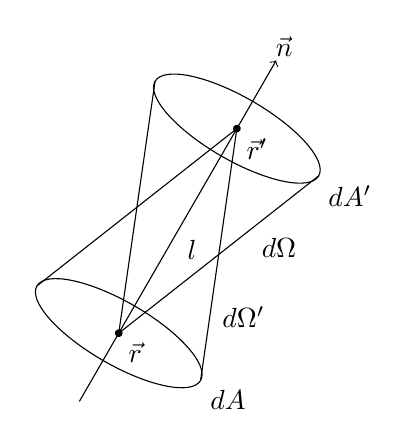
\begin{tikzpicture}
\begin{scope}[rotate=-30]
\fill[black] (0,0) circle [radius=0.05];
\fill[black] (0,3) circle [radius=0.05];
\draw[->] (0,-1) -- (0,4);
\draw(0,0) ellipse [x radius=1.2cm,y radius=0.4cm];
\draw(0,3) ellipse [x radius=1.2cm,y radius=0.4cm];
\draw(0,0) -- (-1.2,3);
\draw(0,0) -- (+1.2,3);
\draw(0,3) -- (-1.2,0);
\draw(0,3) -- (+1.2,0);
\draw (0,4.2) node {$\vec n$};
\draw (0,0) node[below right] {$\vec r$};
\draw (0,3) node[below right] {$\vec r'$};
\draw (1.2,0) node[below right] {$dA$};
\draw (1.2,3) node[below right] {$dA'$};
\draw (0.8,2) node[below right] {$d\Omega$};
\draw (0.8,1) node[below right] {$d\Omega'$};
\draw (0,1.5) node[below right] {$l$};
\end{scope}
\end{tikzpicture}
\end{center}
\caption{The geometry used in the proof of the conservation of specific
  intensity.}
\label{fig-specific-intensity-conservation}
\end{figure}

An important property of the specific intensity is that in free space it
is conserved along a ray. Consider Figure
\ref{fig-specific-intensity-conservation}, which shows two points on a
ray, $\vec r$ and $\vec r' = \vec r + l\vec n$ and two areas at those
points, normal to the ray, $dA$ and $dA'$. We will consider all the
photons in the frequency interval $(\nu,\nu+d\nu)$ that pass through
$dA$ in the time interval $(t,t+dt)$ and later pass through $dA'$ in the
interval $(t',t'+dt)$. Clearly, the photons pass through $dA'$ a time
$l/c$ after they pass through $dA$, so $t'=t+l/c$.

\newslide

In free space, and ignoring the gravitational redshift (see Problem
\ref{problem-gravitational-redshift}), gravitational lensing, and very
rare photon-photon scatterings, the energy carried by these photons will
be conserved. More precisely, the energy $dE$ that passes through $dA$
in the time interval $(t,t+dt)$ in the frequency interval
$(\nu,\nu+d\nu)$, at angles that will take it through $dA'$ will be
equal to the energy $dE'$ that passes through $dA'$ in the time interval
$(t',t'+dt)$ in the frequency interval $(\nu,\nu+d\nu)$ at angles that
took it through $dA$. From the definition of specific intensity we have
\begin{align}
dE = I_\nu(\vec r, \vec n, \nu, t)\,dA\,d\Omega\,d\nu\,dt
\end{align}
and
\begin{align}
dE' = I_\nu(\vec r', \vec n, \nu, t')\,dA'\,d\Omega'\,d\nu\,dt
\end{align}
where $d\Omega$ is the solid angle subtended by $dA'$ at $\vec r$ and
$d\Omega'$ is the solid angle subtended by $dA$ at point $\vec r'$.
Since, $dE = dE'$, we have
\begin{align}
I_\nu(\vec r, \vec n, \nu, t)\,dA\,d\Omega = 
I_\nu(\vec r', \vec n, \nu, t')\,dA'\,d\Omega'.
\end{align}
\newslide
However, $d\Omega = dA'/l^2$ and $d\Omega' = dA/l^2$, and so
\begin{align}
I_\nu(\vec r, \vec n, \nu, t)\,dA\,dA'/l^2 = 
I_\nu(\vec r', \vec n, \nu, t')\,dA'\,dA/l^2.
\end{align}
and
\begin{align}
I_\nu(\vec r, \vec n, \nu, t) = 
I_\nu(\vec r', \vec n, \nu, t'),
\end{align}
or
\begin{align}
I_\nu(\vec r, \vec n, \nu, t) = 
I_\nu(\vec r + l\vec n, \vec n, \nu, t + l/c).
\end{align}
This shows that in the absence of interaction with matter, the specific
intensity is conserved as radiation streams along its path. A few
moments of consideration show that if the radiation field is in
steady state, then
\begin{align}
I_\nu(\vec r, \vec n, \nu, t) = 
I_\nu(\vec r + l\vec n, \vec n, \nu, t),
\end{align}
that is, the specific intensity is constant along straight lines.

\newslide

\subsection{Why Use the Specific Intensity?}

Why do we use the specific intensity rather than some more physically
obvious quantity such as the density of photons or the density of
energy? 

\newslide

First, we need a quantity that encapsulates all of the information about
radiation. The specific intensity contains all of the information
required to describe unpolarized light completely, as it specifies the
quantity of radiation at a given point, in a given direction, at a given
frequency, and at a given time.

\newslide

Second, the conservation of the specific intensity along a ray in the
absence of interaction with matter means that in the transfer of
specific intensity we need only consider changes due to interaction with
matter and ignore changes due to geometry. For example, the density of
photons emitted by a point source into free space decreases as $1/r^2$
simply because of geometric dilution, but the specific intensity remains
the same. This is an enormous simplification.

\newslide

\section{The Photon Distribution Function}

The equivalent of the specific intensity $I_\nu$ in the photon-gas
description is the photon distribution function $f$, the phase space
density of photons. Phase space is a six-dimensional space specified by
the three components of position and the three components of momentum.
The photon distribution function $f(\vec r, \vec p, t)$ is such that the
number of photons $dN$ in a volume of real space $d \vec r$ and volume of
momentum space $d\vec p$ centered on position $\vec r$ and momentum
$\vec p$ is given by
\begin{align}
dN = f(\vec r, \vec p, t)\,d\vec r\,d\vec p.
\end{align}

\newslide

\begin{figure}
\begin{center}
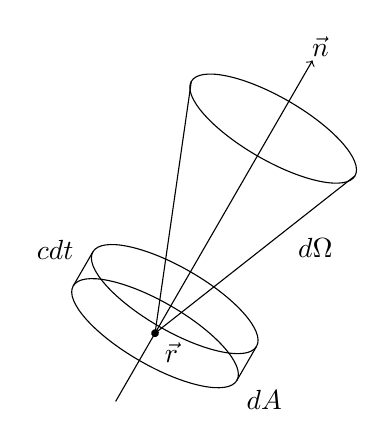
\begin{tikzpicture}
\begin{scope}[rotate=-30]
\fill[black] (0,0) circle [radius=0.05];
\draw[->] (0,-1) -- (0,4);
\draw(0,0) ellipse [x radius=1.2cm,y radius=0.4cm];
\draw(0,0.5) ellipse [x radius=1.2cm,y radius=0.4cm];
\draw(+1.2,0.5) -- (+1.2,0);
\draw(-1.2,0.5) -- (-1.2,0);
\draw(0,3) ellipse [x radius=1.2cm,y radius=0.4cm];
\draw(0,0) -- (-1.2,3);
\draw(0,0) -- (+1.2,3);
\draw (0,4.2) node {$\vec n$};
\draw (0,0) node[below right] {$\vec r$};
\draw (1.2,0) node[below right] {$dA$};
\draw (0.8,2) node[below right] {$d\Omega$};
\draw (-1.2,0.25) node[above left] {$cdt$};
\end{scope}
\end{tikzpicture}
\end{center}
\caption{The geometry used in the determination of the relation between
  the photon distribution function $f$ and the specific intensity
  $I_\nu$.}
\label{fig-photon-distribution-function}
\end{figure}

We'll now develop the relation between $f$ to $I_\nu$. Consider
Figure~\ref{fig-photon-distribution-function}. We know from the
definition of the specific intensity that the energy $dE$ transported by
radiation across an area $dA$, centered on $\vec r$ and perpendicular to
$\vec n$, into a solid angle $d\Omega$ about $\vec n$, in a frequency
interval $(\nu,
\nu+d\nu)$, in a time interval $(t,t+dt)$ is given by
\begin{align}
dE = I_\nu(\vec r, \vec n, \nu, t)\,dA\,d\Omega\,d\nu\,dt.
\end{align}
In terms of the photon distribution function, 
\begin{align}
dE = h\nu f\,d\vec r\,d\vec p,
\end{align}
where the volume of phase space $d\vec r\,d\vec p$ contains the all of
the photons that pass through an area $dA$, centered on $\vec r$ and
perpendicular to $\vec n$, into a solid angle $d\Omega$ about $\vec n$,
in a frequency interval $(\nu, \nu+d\nu)$, in a time interval
$(t,t+dt)$. Since photons travel a distance $c dt$ in time $dt$, we have
\begin{align}
d\vec r = c\,dt\,dA.
\end{align}
Furthermore, since the momentum of a photon is $p = h\nu/c$, the photons
traveling into a solid angle $d\Omega$ in a frequency
interval $(\nu,
\nu+d\nu)$ are those in the partial shell in momentum space between
$(p,p+dp)$ with directions in $d\Omega$. That is,
\begin{align}
d\vec p = p^2\,dp\,d\Omega = \frac{h^3\nu^2}{c^3}\,d\nu\,d\Omega.
\end{align}
Thus, 
\begin{align}
dE = I_\nu(\vec r, \vec n, \nu, t)\,dA\,d\Omega\,d\nu\,dt
= \frac{h^4\nu^3}{c^2}f\,dA\,d\Omega\,d\nu\,dt,
\end{align}
and so
\begin{align}
I_\nu(\vec r, \vec n, \nu, t)
= \frac{h^4\nu^3}{c^2}f.
\end{align}

Like the specific intensity, the photon distribution function also
completely describes unpolarized light and also is conserved along a
ray. However, the specific intensity is often preferred because it is
more directly related to macroscopic thermodynamic quantities, such as
energy and temperature.

Distribution functions are commonly used in physics and astrophysics,
for example, in the statistical mechanics of gases and in the dynamics
of stellar systems; they are all defined in terms of the number density of the relevant particle in phase space. A standard result for distribution functions is that they are
conserved along a path under certain conditions. Thus, we can think of the conservation of
$I_\nu$ along a ray as coming from the conservation of $f$ (and $\nu$)
along the same ray. (Similarly, we can consider the equation of
radiation transfer that we will derive in chapter~\ref{chapter:interaction} as a collisional
Boltzmann equation for $f$.)

\newslide

\section{The Moments of the Specific Intensity}

The moments of the specific intensity with respect to the direction
vector $\vec n$ are doubly useful, as they have physical meaning (such
as the energy, the energy flux, and the radiation pressure) and are used
in the development of solutions for the equations of radiative transfer.
In dyadic form, the $m$-th moment is defined as
\begin{align}
M_m(I_\nu) \equiv \frac{1}{4\pi} \int_{4\pi}\!\!\!d\Omega\:
I_\nu(\vec r, \vec n, \nu, t) \vec n^m.
\end{align}
In general the zeroth moment is a scalar, the first moment is a vector, and the
second moment is a symmetric tensor of rank 2. In component form, these moments are
\begin{align}
M_0(I_\nu)_{\phantom{ij}}
&\equiv 
\frac{1}{4\pi} \int_{4\pi}\!\!\!d\Omega\:
I_\nu(\vec r, \vec n, \nu, t),\\
M_1(I_\nu)_{i\phantom{j}}
&\equiv 
\frac{1}{4\pi} \int_{4\pi}\!\!\!d\Omega\:
I_\nu(\vec r, \vec n, \nu, t) n_i,\\
\intertext{and}
M_2(I_\nu)_{ij}
&\equiv 
\frac{1}{4\pi} 
\int_{4\pi}\!\!\!d\Omega\:
I_\nu(\vec r, \vec n, \nu, t) n_i n_j.
\end{align}
Here, $n_i$ and $n_j$ are Cartesian components of $\vec n$.

\newslide

We often work in a plane-parallel symmetry, which allows us to simplify the first and second moments considerably. If
we take the $z$ axis to be the vertical axis of the plane-parallel
symmetry, then we have
reflectional symmetry about the planes $x = 0$ and $y = 0$ and
rotational symmetry about the $z$ axis. 

Consider the $x$ component of the first moment, $M_1(I_\nu)_x$. This is given by
\begin{align}
M_1(I_\nu)_x = \frac{1}{4\pi}\int_{4\pi}\!\!\!d\Omega\:
I_\nu(n_x, n_y) n_x,
\end{align}
where we indicate the explicit dependence on the components $n_x$ and $n_y$ of $\vec n$. There is no corresponding explicit dependence on $n_z$, since $n_z$ is given implicity in terms of $n_x$ and $n_y$ by $n_x^2+n_y^2+n_z^2=1$. We omit the implicit dependence on $\vec r$, $\nu$, and $t$ for conciseness. We can split the integral into two hemispheres,
\begin{align}
M_1(I_\nu)_x =
\frac{1}{4\pi}\left[
\int_{n_x > 0}\!\!\!\!\!\!\!\!\!d\Omega\: I_\nu(n_x, n_y) n_x
+
\int_{n_x < 0}\!\!\!\!\!\!\!\!\!d\Omega\: I_\nu(n_x, n_y) n_x
\right].
\end{align}
We then make the substitution $n_x'=-n_x$ in the second integral.
\begin{align}
M_1(I_\nu)_x = \frac{1}{4\pi}\left[
\int_{n_x > 0}\!\!\!\!\!\!\!\!\!d\Omega\: I_\nu(n_x, n_y) n_x
-
\int_{n_x' > 0}\!\!\!\!\!\!\!\!\!d\Omega'\: I_\nu(-n_x', n_y) n_x'
\right].
\end{align}
We then note that the reflectional symmetry through the plane $n_x = 0$ implies that
\begin{align}
I_\nu(n_x, n_y) = I_\nu(-n_x, n_y),
\end{align}
and so the two integrals cancel, leaving
\begin{align}
M_1(I_\nu)_x = 0.
\end{align}

\newslide

We can make a similar argument using the reflectional symmetry through the plane $n_y = 0$ to show that the $y$ component $M_1(I_\nu)_y$ is also zero. However, in plane-parallel symmetry we do not in general have symmetry through the plane $z = 0$, and so in general the $z$ component $M_1(I_\nu)_z$ is not zero. Thus, we can fully specify the vector first moment by its $z$
component, $M_1(I_\nu)_z$, the only component that is not identically
zero. That is, we have,
\begin{align}
M_1(I_\nu)_x &= 
M_1(I_\nu)_y = 0\\
\intertext{and}
M_1(I_\nu)_z &= \frac{1}{4\pi} \int_{4\pi}\!\!\!d\Omega\:
I_\nu(\vec r, \vec n, \nu, t) n_z.
\end{align}

More intuitively, we could argue that in plane-parallel symmetry, any vector must be either parallel or anti-parallel to the $z$ axis. Thus, the $x$ and $y$ components of the first moment must be zero.

\newslide

Similarly, consideration of the second moment shows that the
off-diagonal components must be zero. Rotational symmetry about the $z$ axis further implies  that the $xx$ and $yy$
components must be equal. Finally, we note that $\vec n$ is a unit
vector, so $n_x^2 + n_y^2 + n_z^2 = 1$, and so the trace of the second
moment satisfies $M_2(I_\nu)_{xx} + M_2(I_\nu)_{yy} + M_2(I_\nu)_{zz} =
M_0(I_\nu)$. Thus, we can fully specify the tensor second moment by
$M_2(I_\nu)_{zz}$ and $M_0(I_\nu)$ as
\begin{align}
M_2(I_\nu)_{xx} &= 
M_2(I_\nu)_{yy} = \frac{1}{2}(M_0(I_\nu) - M_2(I_\nu)_{zz}),\\
\intertext{and}
M_2(I_\nu)_{zz} &= \frac{1}{4\pi} \int_{4\pi}\!\!\!d\Omega\:
I_\nu(\vec r, \vec n, \nu, t) n_z n_z.
\end{align}

\newslide

To summarize, in plane-parallel symmetry the first three moments
are fully-specified by the values of $M_0(I_\nu)$, $M_1(I_\nu)_z$, and
$M_2(I_\nu)_{zz}$. We normally write these as $J_\nu$, $H_\nu$, and
$K_\nu$, where
\begin{align}
J_\nu &\equiv M_0(I_\nu)_{\phantom{ij}}
\equiv 
\frac{1}{4\pi} \int_{4\pi}\!\!\!d\Omega\:
I_\nu(\vec r, \vec n, \nu, t),\\
H_\nu &\equiv M_1(I_\nu)_{z\phantom{j}}
\equiv 
\frac{1}{4\pi} \int_{4\pi}\!\!\!d\Omega\:
I_\nu(\vec r, \vec n, \nu, t) n_z,\\
\intertext{and}
K_\nu &\equiv M_2(I_\nu)_{zz}
\equiv 
\frac{1}{4\pi} 
\int_{4\pi}\!\!\!d\Omega\:
I_\nu(\vec r, \vec n, \nu, t) n_z^2.
\end{align}

\newslide

In spherical symmetry, we can construct a local cartesian coordinate system with the $z$ axis parallel to the local radial axis. This local cartesian coordinate system then has reflectional symmetry about the planes $x = 0$ and $y = 0$ and rotational symmetry about the $z$ axis. These were precisely the symmetries we used above in plane-parallel symmetry to show that we could reduce the first three moments to three components. We can see, therefore, that in spherical symmetry we can do the same.

\newslide

To integrate over solid angle, we change variables to the polar angle
$\theta$ between $\vec n$ and the $z$ axis and the azimuthal angle
$\phi$ (see Figure
\ref{fig-dOmega}), and so have
\begin{align}
\frac{1}{4\pi}
\int_{4\pi}\!\!\!d\Omega =
\frac{1}{4\pi}
\int_0^{2\pi}\!\!\!d\phi\int_0^\pi\!\!\!d\theta\:
\sin\theta.
\end{align}
\begin{figure}
\begin{center}
\begin{tikzpicture}[scale=0.7,rotate around x=-90,rotate around z=-90]
\draw[->] (0,0,0) -- (6,0,0) node [at end,left] {$x$};
\draw[->] (0,0,0) -- (0,6,0) node [at end,right] {$y$};
\draw[->] (0,0,0) -- (0,0,6) node [at end,left] {$z$};
\begin{scope}[rotate around y=-90,rotate around x=-30]
\draw(0,0) -- (4,3) -- (0,3) -- (0,0);
\begin{scope}[rotate around z={atan(3/4)},rotate around x=0]
\draw[->] (5,0.25,1.5) node [anchor=200] {$d\theta$} -- (5,0.25,0.5);
\draw[->](5,-0.75,0.25) node [above] {$d\phi\sin\theta$} -- (5,0,0.25);
\draw
  (5,0,0) -- 
  (5,0.5,0) --
  (5,0.5,0.5) -- 
  (5,0,0.5) -- 
  cycle;  
\end{scope}
\draw[->] (2,0) 
  arc [start angle=0,end angle={0.5*atan(3/4)},radius=2] 
  node[above] {$\theta$}
  arc [start angle={0.5*atan(3/4)},end angle={atan(3/4)},radius=2];
\end{scope}
\draw[->](2,0) 
  arc [start angle=0,end angle=30,radius=2] 
  node [below] {$\phi$}
  arc [start angle=30,end angle=60,radius=2] 
  ;
\end{tikzpicture}
\end{center}
\caption{The element of solid angle $d\Omega$ is equal to $\sin\theta\,d\theta
\,d\phi$.}
\label{fig-dOmega}
\end{figure}

\newslide

In plane-parallel symmetry, we have rotational symmetry
about the $z$ axis, which allows us to integrate over $\phi$ directly,
giving
\begin{align}
\frac{1}{4\pi}
\int_{4\pi}\!\!\!d\Omega =
\frac{1}{2}\int_0^\pi\!\!\!d\theta\:
\sin\theta.
\end{align}
The substitution $\mu \equiv \cos\theta$ allows this integral to be
expressed in an especially simple form. Instead of $\theta$ varying from
0 to $\pi$, we then have $\mu$ varying from $+1$ to $-1$, with $\mu =
+1$ being parallel to the symmetry axis ($\theta = 0$), $\mu = 0$ being
perpendicular to the symmetry axis ($\theta =
\pi/2$), and $\mu = -1$ being anti-parallel to the symmetry axis ($\theta
= \pi$). Since $d\mu =
\sin\theta\,d\theta$, we obtain
\begin{align}
\frac{1}{4\pi}
\int_{4\pi}\!\!\!d\Omega =
\frac{1}{2} \int_{-1}^{+1} \!\!\!d\mu.
\end{align}
This integration over $\phi$ and substitution of $\mu$ for $\theta$ is a
very common trick when we have plane-parallel geometry. 

\newslide

Returning to the moments, we have $n_z = \cos \theta = \mu$, so
\begin{align}
J_\nu &= \frac{1}{2} \int_{-1}^{+1} \!\!\!d\mu\:I_\nu(\mu),\\
H_\nu &= \frac{1}{2} \int_{-1}^{+1} \!\!\!d\mu\:I_\nu(\mu)\mu,
\intertext{and}
K_\nu &= \frac{1}{2} \int_{-1}^{+1} \!\!\!d\mu\:I_\nu(\mu)\mu^2.
\end{align}
That is, we can interpret $J_\nu$, $H_\nu$, and $K_\nu$ as the first
three moments of $I_\nu$ with respect to $\mu$. We now consider physical
interpretations of these moments.

\newslide

\subsection{Zeroth Moments}

\newslide

\subsubsection{The Mean Intensity}

The zeroth moment $J_\nu$ or mean intensity is defined above as
\begin{align}
J_\nu = \frac{1}{2}
\int_{-1}^{+1}\!\!\!d\mu\:I_\nu.
\end{align}
Physically, $J_\nu$ is just the angular mean of the specific intensity.
If $I_\nu$ is isotropic, then $J_\nu = I_\nu$.

\newslide

\subsubsection{The Photon Density}

The monochromatic density $N_\nu$ of photons per unit
frequency is given by
\begin{align}
N_\nu = \frac{4\pi J_\nu}{h\nu c}.
\end{align}
and the total photon density $N$ is given by
\begin{align}
N = \frac{4\pi}{hc} \int_0^\infty\!\!\!d\nu\: \frac{J_\nu}{\nu}.
\end{align}
These expressions are derived in Problem
\ref{problem-photon-density}. 

\newslide

\subsubsection{The Energy Density}

The monochromatic energy density $u_\nu$ per unit frequency
is given by
\begin{align}
u_\nu = \frac{4\pi J_\nu}{c}.
\end{align}
and the total energy density $E$ is given by
\begin{align}
u = \frac{4\pi J}{c}.
\end{align}
These expressions are derived in Problem
\ref{problem-energy-density}. 

\newslide

\subsection{First Moments}

\newslide

\subsubsection{The Eddington Flux}

The first moment $H_\nu$ or Eddington flux is defined above as
\begin{align}
H_\nu = \frac{1}{2} \int_{-1}^{+1}\!\!\!d\mu\:\mu I_\nu.
\end{align}
The Eddington flux has no direct physical interpretation, but it is
widely used in solutions to the radiation transfer problem. If $I_\nu$
is isotropic, then $H_\nu = 0$.

\newslide

\subsubsection{The Energy Flux}

\begin{figure}
\begin{center}
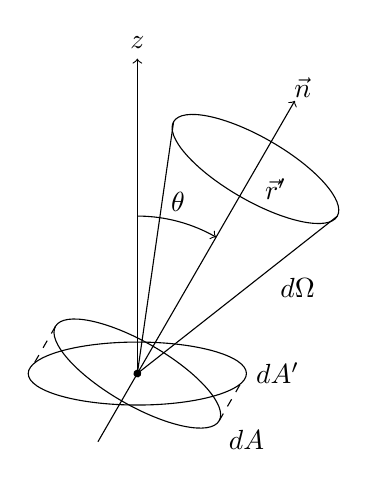
\begin{tikzpicture}
\begin{scope}[rotate=-30]
\fill[black] (0,0) circle [radius=0.05];
\draw[->] (0,-1) -- (0,4);
\draw(0,0) ellipse [x radius=1.2,y radius=0.4];
\draw(0,3) ellipse [x radius=1.2,y radius=0.4];
\draw(0,0) -- (-1.2,3);
\draw(0,0) -- (+1.2,3);
\draw (0,4.2) node {$\vec n$};
\draw (0,3) node[below right] {$\vec r'$};
\draw (1.2,0) node[below right] {$dA$};
\draw (0.8,2) node[below right] {$d\Omega$};
\draw[dashed](+1.2,0) -- (+1.2,{+1.2*sin(30)});
\draw[dashed](-1.2,0) -- (-1.2,{-1.2*sin(30)});
\end{scope}
\draw[->] (0,0) -- (0,4) node[above] {$z$};
\draw(0,0) ellipse [x radius={1.2/cos(30)},y radius=0.4];
\draw ({1.2/cos(30)},0) node[right] {$dA'$};

\draw[->]
  (0,2) 
  arc [start angle=90,end angle=75,radius=2]
  node [above] {$\theta$}
  arc [start angle=75,end angle=60,radius=2]
  ;
\end{tikzpicture}
\end{center}
\caption{The geometry used in the derivation of the flux.}
\label{fig-flux}
\end{figure}

Consider Figure \ref{fig-flux}. 
We define the energy flux $F_\nu$ such that the energy $dE$ that flows through area
$dA'$ perpendicular to the $z$-axis, into all solid angles, in frequency interval $(\nu,\nu+d\nu)$, in
time interval $(t,t+dt)$ is
\begin{align}
dE \equiv F_\nu(\vec r, \nu, t) dA' d\nu dt.
\end{align}

\newslide

From the definition of
specific intensity, 
we have
\begin{align}
dE = 
\int_{4\pi}\!\!\!d\Omega\:
I_\nu(\vec r, \nu, t) dA d\nu dt,
\end{align}
in which $dA$ is the projection of $dA'$ onto a plane perpendicular to the $\vec n$. 
The two areas
are related by
\begin{align}
dA = dA' \cos\theta,
\end{align}
where $\theta$ is the angle between $\vec n$ and the
$z$-axis. Thus, equating the two expressions for $dE$, we have
\begin{align}
F_\nu = \int_{4\pi}\!\!\!d\Omega\:
I_\nu(\vec r, \vec n, \nu, t) \cos\theta.
\end{align}
This is proportional to the first-moment, and so we have
\begin{align}
F_\nu = 4\pi H_\nu =
2\pi \int_{-1}^{+1}\!\!\!d\mu\:\mu I_\nu.
\end{align}
The total energy flux $F = \int_0^\infty\!\!\!d\nu F_\nu = 4\pi H$ is
one of the most important quantities in an atmosphere. We use it so much that we often refer to it simply as ``the'' flux.

\newslide

If $I_\nu$ is isotropic, then $F_\nu = 0$. This result simply states
that if the specific intensity is isotropic, then there is no net flux
of energy. This is to expected on symmetry grounds; an isotropic
specific intensity has no preferred direction in which energy might flow.

\newslide

If $I_\nu$ is isotropic over the outward hemisphere and zero
over the inward hemisphere, for example, if a flat surface
of constant brightness is emitting into free space, then we
have
\begin{align}
I_\nu(\mu) =
\begin{cases}
I_\nu(1)&\mbox{for $\mu>0$,}\\
0&\mbox{for $\mu<0$,}
\end{cases}
\end{align}
and the flux is given by 
\begin{align}
\label{eq-flux-from-surface}
F_\nu = \pi I_\nu(1).
\end{align}
This expression is derived in Problem \ref{problem-flux-from-surface}.
This expression for the flux leads to the use of the quantity
$F_\nu/\pi$, which is called the ``astrophysical flux'' in contrast to
the ``physical flux'' $F_\nu$. The astrophysical flux would be of
largely historical interest were it not that the emergent flux of a
model atmospheres is most often tabulated in terms of the astrophysical
flux $F_\nu/\pi$ rather than the energy flux $F_\nu$. For example,
Kurucz distributes tables of astrophysical fluxes for his model
atmospheres. Note that some authors, in particular
\cite{Chandrasekhar-1960}, \cite{Mihalas-1978}, \cite{Gray-1992}, use
the symbol $F_\nu$ for the astrophysical flux and either $\pi F_\nu$ or
the symbol $\mathcal{F}_\nu$ for the physical flux, but here we follow
\cite{Milne-1930} and \cite{Rybicki-1979} in using $F_\nu$ for the
physical flux.

\newslide

\subsubsection{The Photon Flux}

We can generalize the definition of a flux so that the ``flux of $X$'' such that the quantity $dX$ that flows through area
$dA'$ perpendicular to the $z$-axis, into all solid angles, in frequency interval $(\nu,\nu+d\nu)$, in
time interval $(t,t+dt)$ is
\begin{align}
dX \equiv F_X(\vec r, \nu, t) dA' d\nu dt.
\end{align}

A simple application is to define the photon flux as the number of photons that flow through an area perpendicular to the $z$ axis, in a frequency interval, and in
a time interval.
Since energy is carried by photons and since each photon has an energy
$h\nu$, the photon flux is related to the energy flux and
is given by
\begin{align}
\frac{1}{h\nu} F_\nu. 
\end{align}

\newslide

\subsection{Second Moments}

\newslide

\subsubsection{The Eddington Pressure}

The second moment $K_\nu$ or Eddington pressure is defined above as
\begin{align}
K_\nu = \frac{1}{2} \int_{-1}^{+1}\!\!\!d\mu\:I_\nu\mu^2.
\end{align}
Like the Eddington flux,
the Eddington pressure has no direct physical
interpretation, but it is widely used in solutions to the
radiation transfer problem. 

The ratio
\begin{align}
f \equiv \frac{K_\nu}{J_\nu}
\end{align}
is known as the Eddington factor. (Although the same symbol is used for
both the Eddington factor and the photon distribution function, they are
used in very different contexts and no real ambiguity should arise.) If
$I_\nu$ is isotropic, then $K_\nu = I_\nu / 3$, and the Eddington factor
is 1/3. For a non-isotropic radiation field, the Eddington factor will
not in general be 1/3, but will always satisfy in $0
\le f \le 1$.

\newslide

\subsubsection{The Radiation Pressure}

The radiation pressure is defined as the flux of momentum in the
radiation field. The flux of momentum is the flux of a vector quantity
and so in general will be a second-rank tensor. However, as we saw
above, if we have rotational symmetry, the tensor can be essentially
reduced to a scalar quantity: the flux parallel to the symmetry axis
(i.e., upwards or outwards) of the component of momentum parallel to the
symmetry axis. We often refer to this component as \emph{the} radiation pressure $p_\nu$, ignoring the other components.
 
\newslide

We normally consider pressure to be the force per unit area
exerted on the walls of a vessel by the fluid contained
within the vessel rather than the flux of momentum. The two
quantities have the same units and are clearly related,
because the force on the walls is derived from the change in
momentum of the particles when they impinge on the walls. If the interactions between the particles and the walls are elastic, then the force per unit area is equal to the flux perpendicular to the wall of the component of momentum perpendicular to the wall. However, if the interaction is more complex (e.g., if the particles stick to the wall or are absorbed rather than interacting elastically), the relation between the force per unit area and the flux of momentum is more complex. This is particularly relevant to photons, since in general they do not interact elastically with matter but rather are more typically absorbed. Given this, it is preferable here to define the radiation pressure to be the flux of momentum and to calculate separately the force on matter interacting with this radiation, taking the physics of the of the interaction explicitly into account.

%This is explored in more detail in Problem
%\ref{problem-radiation-pressure}.

\newslide

Consider Figure
\ref{fig-flux} again, and recall that the energy carried by
radiation across $dA'$ is $I_\nu
\cos\theta dA d\Omega d\nu dt$. The $z$-component of
momentum carried by radiation across the same area is
\begin{align}
I_\nu \cos^2\theta dA d\Omega d\nu dt / c,
\end{align}
where the factor of
$1/c$ relates the momentum of a photon to its energy and the
additional factor of $\cos\theta$ comes from considering
just the component of the momentum of a photon parallel to
the $z$-axis. From this, we can see that the radiation
pressure $p_\nu$ is given by
\begin{align}
p_\nu = \frac{1}{c} \int_{4\pi}\!\!\!d\Omega\:I_\nu
\cos^2\theta.
\end{align}
Again, we see that this is related to the second moment of
$I_\nu$, and we have
\begin{align}
p_\nu= \frac{4\pi}{c} K_\nu =
\frac{2\pi}{c} \int_{-1}^{+1}\!\!\!d\mu\:\mu^2 I_\nu.
\end{align}
If $I_\nu$ is isotropic, then $p_\nu = {4\pi J_\nu / 3c}$.

\newslide

We can interpret the Eddington factor $f$ as the ratio
of the monochromatic pressure to the monochromatic energy
density $p_\nu/u_\nu$, because $p_\nu$ and $u_\nu$ are
simply $K_\nu$ and $J_\nu$ multiplied by the same factor of
$4\pi/c$. From classical thermodynamics, we know that the
ratio of pressure to internal energy is $\gamma - 1$, in
which $\gamma$ is the ratio of the specific heats $c_p/c_V$.
Thus, an isotropic radiation field has $\gamma = 4/3$.

However, isotropic radiation is a special case. In general,
the Eddington factor and hence the ratio of the pressure to
the internal energy depend on the degree of anisotropy in
the radiation field and can range from 0 to 1. This has an
analogy in gases of massive particles: an ideal gas of
massive particles has an isotropic distribution of
velocities when at rest and the ratio of pressure to
internal thermal energy is 2/3; however, when the gas is has
a bulk motion, the velocity distribution is not isotropic
and the ratio of ram pressure to bulk kinetic energy varies
from 0 to 1/2 depending on the direction of the flow.

\newslide

\section{Black-Body Radiation}


In thermodynamic equilibrium at a temperature $T$, the
radiation field is uniform, time-independent, and has a
frequency distribution given by the Planck functions,
$I_\nu^* = B_\nu$ and $I_\lambda^* = B_\lambda$ where
\begin{align}
B_\nu &\equiv \frac{2 h \nu^3}{c^2}
(e^{h\nu/kT} -1)^{-1},
\\
\intertext{and}
B_\lambda &\equiv \frac{2 h c^2}{\lambda ^5}
(e^{hc/kT\lambda} -1)^{-1}.
\end{align}
Such radiation is known as ``black-body'' radiation. It is conventional
to use the superscript $^*$ to denote the value of physical quantities
in equilibrium.

\newslide

\begin{figure}
\footnotesize
\begin{tikzpicture}
\begin{axis}[
   xlabel={$\log_{10} \nu\:[\mathrm{Hz}]$},
   ylabel={$\log_{10} B_\nu\:[\mathrm{W\,s^{-1}\,m^{-2}\,Hz^{-1}\,sr^{-1}}]$},
   ymin=-12,
   ymax=-4,
   minor y tick num=3,
   xmin=12.5,
   xmax=16.5,
   minor x tick num=4,
]
\addplot[black] table[x index=0,y index=1]{chapter-2/B-nu.tsv};
\addplot[black] table[x index=0,y index=2]{chapter-2/B-nu.tsv};
\addplot[black] table[x index=0,y index=3]{chapter-2/B-nu.tsv};
\addplot[black] table[x index=0,y index=4]{chapter-2/B-nu.tsv};
\addplot[black] table[x index=0,y index=5]{chapter-2/B-nu.tsv};
\end{axis}
\end{tikzpicture}
\caption{The Planck function $B_\nu$ at temperatures of (bottom to top)
  2500~K, 5000~K, 10,000~K, 20,000~K, and 40,000~K. A frequency of
  $10^{14.5}$~Hz corresponds to a wavelength of about 1~{\micron}.}
\label{figure-B-nu}
\end{figure}

\begin{figure}
\footnotesize
\begin{tikzpicture}
\begin{axis}[
   xlabel={$\log_{10} \lambda\:[\mathrm{\micron}]$},
   ylabel={$\log_{10} B_\lambda\:[\mathrm{W\,m^{-2}\,\micron^{-1}\,sr^{-1}}]$},
   ymin=0,
   ymax=15,
   minor y tick num=3,
   xmin=-2.5,
   xmax=2.5,
   minor x tick num=4,
]
\addplot[black] table[x index=0,y index=1]{chapter-2/B-lambda.tsv};
\addplot[black] table[x index=0,y index=2]{chapter-2/B-lambda.tsv};
\addplot[black] table[x index=0,y index=3]{chapter-2/B-lambda.tsv};
\addplot[black] table[x index=0,y index=4]{chapter-2/B-lambda.tsv};
\addplot[black] table[x index=0,y index=5]{chapter-2/B-lambda.tsv};
\end{axis}
\end{tikzpicture}
\caption{The Planck function $B_\lambda$ at temperatures of (bottom to
  top) 2500~K, 5000~K, 10000~K, 20000~K, and 40000~K.}
\label{figure-B-lambda}
\end{figure}
Figures \ref{figure-B-nu} and \ref{figure-B-lambda} show the Planck
functions $B_\nu$ and $B_\lambda$ at temperatures, frequencies, and
wavelengths of relevance for stellar atmospheres. The figures illustrate
the monotonic increase in the Planck functions with temperature at a
given frequency or wavelength. They also show the two important limiting
cases of the Planck functions, the low-frequency Rayleigh-Jeans tail for
$h\nu \ll kT$, which has
\begin{align}
B_\nu \approx \frac{2kT}{c^2} \nu^2,
\end{align}
and the high-frequency Wien tail for $h\nu \gg kT$, which has 
\begin{align}
B_\nu \approx \frac{2 h \nu^3}{c^2} e^{-h\nu/kT}.
\end{align}
In the Rayleigh-Jeans tail, the Planck function changes only linearly
with temperature at a given frequency, whereas in the Wien tail the
change with temperature is much more dramatic. We will see, however,
that the dominant radiation in an atmosphere often has $h\nu \sim kT$,
close to the peak of $B_\nu$, in which case we must use the exact
expression for $B_\nu$.

\newslide

Since black-body radiation is isotropic we have
\begin{align}
J_\nu^* = I_\nu^* = B_\nu,
\end{align}
\begin{align}
F_\nu^* = 0,
\end{align}
and
\begin{align}
p_\nu^* = \frac{4\pi}{3c} I_\nu = \frac{4\pi}{3c} B_\nu.
\end{align}

\newslide

The total mean intensity is
\begin{align}
J^* = B = \int_0^\infty
B_\nu\,d\nu
\end{align}
If substitute for $B_\nu$ and then use $x \equiv h\nu / kT$,
we find
\begin{align}
B = \left(\frac{2 k^4}{c^2 h^3}\right) T^4 \int_0^\infty\!\!\!dx\: x^3(e^x -
1)^{-1}.
\end{align}
The integral is a pure number, and can be shown to have the
value $\pi^4/15$. Thus
\begin{align}
B = \left(\frac{2 \pi^4 k^4}{15 c^2 h^3}\right)T^4.
\end{align}
The total energy density is
\begin{align}
u^* = \frac{4\pi}{c} J^* = \frac{4\pi}{c} B = a T^4,
\end{align}
in which $a \equiv 8 \pi^5 k^4 / 15 c^3 h^3$ is the radiation constant.
This result can also be obtained by consideration of the thermodynamics
of black-body radiation \citep[pp.\ 17--18]{Rybicki-1979}.

\newslide

If a surface emits as a black body, i.e., has $I_\nu = B_\nu$ over
the outward hemisphere and has $I_\nu = 0$ over the inward hemisphere,
then by equation \ref{eq-flux-from-surface} the flux is $F_\nu
= \pi B_\nu,$ and the total flux is 
\begin{align}
F = \pi B
= \sigma T^4,
\label{equation:flux-from-black-body}
\end{align}
in which $\sigma \equiv ac / 4$ is the Stefan-Boltzmann constant,
$\sigma \equiv (2\pi^5k^4)/(15c^2h^3) = 5.670 \times
10^{-5}\space\mathrm{erg~s^{-1}~cm^{-2}~K^{-4}}$.

\newslide

\section{The Effective Temperature}

We commonly use the \emph{effective temperature} $\Teff$ as a surrogate
for the total flux in an atmosphere. The effective temperature is
defined in terms of the total flux $F$ by
\begin{align}
F \equiv \sigma \Teff^4.
\label{eq-effective-temperature}
\end{align}
The motivation for this definition is that, as we saw in equation
\ref{equation:flux-from-black-body}, the total flux from a surface that
emits as a black body with a temperature $T$ is $\sigma T^4$.
Nevertheless, we need to be clear that specifying the effective
temperature is simply a different means to give the total flux; the
effective temperature is not a real thermodynamic temperature and does
not imply that the matter in the atmosphere is in thermodynamic
equilibrium.

\newslide

\section{Magnitudes and Colors}

\begin{figure}
\footnotesize
\begin{tikzpicture}
\begin{axis}[
   xlabel={$\lambda\:[\mathrm{nm}]$},
   ylabel={Normalized $S$},
   ymin=0,
   ymax=1,
   minor y tick num=3,
   xmin=300,
   xmax=1100,
   minor x tick num=3,
]
\addplot[black] table {chapter-2/Johnson-Cousins-U.tsv};
\addplot[black] table {chapter-2/Johnson-Cousins-B.tsv};
\addplot[black] table {chapter-2/Johnson-Cousins-V.tsv};
\addplot[black] table {chapter-2/Johnson-Cousins-R.tsv};
\addplot[black] table {chapter-2/Johnson-Cousins-I.tsv};
\end{axis}
\end{tikzpicture}
\caption{The normalized system response $S$ of the Johnson-Cousins $UBVRI$ filters \citep{Bessell-1990}, excluding the atmosphere.}
\label{figure-S-UBVRI}
\end{figure}

\begin{figure}
\footnotesize
\begin{tikzpicture}
\begin{axis}[
   xlabel={$\lambda\:[\mathrm{nm}]$},
   ylabel={Normalized $S$},
   ymin=0,
   ymax=1,
   minor y tick num=3,
   xmin=300,
   xmax=1100,
   minor x tick num=3,
]
\addplot[black] table {chapter-2/Stroemgren-u.tsv};
\addplot[black] table {chapter-2/Stroemgren-v.tsv};
\addplot[black] table {chapter-2/Stroemgren-b.tsv};
\addplot[black] table {chapter-2/Stroemgren-y.tsv};
%\addplot[black] table{figures/crawford-n.dat};
%\addplot[black] table{figures/crawford-w.dat};
\end{axis}
\end{tikzpicture}
\caption{The normalized system response $S$ of the Strömgren $uvby$ filters \citep{Bessell-2011}, excluding the atmosphere.
%and the Crawford $\beta_n$ and $\beta_w$ filters \citep{Crawford-1966}, excluding the atmosphere.
}
\label{figure-S-uvby}
\end{figure}

\begin{figure}
\footnotesize
\begin{tikzpicture}
\begin{axis}[
   xlabel={$\lambda\:[\mathrm{nm}]$},
   ylabel={$S$},
   ymin=0,
   ymax=1.0,
   minor y tick num=3,
   xmin=300,
   xmax=1100,
   minor x tick num=3,
]
\addplot[black] table{chapter-2/SDSS-u.tsv};
\addplot[black] table{chapter-2/SDSS-g.tsv};
\addplot[black] table{chapter-2/SDSS-r.tsv};
\addplot[black] table{chapter-2/SDSS-i.tsv};
\addplot[black] table{chapter-2/SDSS-z.tsv};
\end{axis}
\end{tikzpicture}
\caption{The absolute system response $S$ of the SDSS $u'g'r'i'z'$ filters  at an airmass of 1.3 \citep{Doi-2010}.}
\label{figure-S-ugriz}
\end{figure}

\begin{figure}
\footnotesize
\begin{tikzpicture}
\begin{axis}[
   xlabel={$\lambda\:[\mathrm{nm}]$},
   ylabel={$S$},
   ymin=0,
   ymax=1.0,
   minor y tick num=3,
   xmin=300,
   xmax=1100,
   minor x tick num=3,
]
\addplot[black] table {chapter-2/Pan-STARRS-g.tsv};
\addplot[black] table {chapter-2/Pan-STARRS-r.tsv};
\addplot[black] table {chapter-2/Pan-STARRS-i.tsv};
\addplot[black] table {chapter-2/Pan-STARRS-z.tsv};
\addplot[black] table {chapter-2/Pan-STARRS-y.tsv};
\end{axis}
\end{tikzpicture}
\caption{The absolute system response $S$ of the Pan-STARRS1 $grizy$ filters  at an airmass of 1.2 \citep{Tonry-2012}.}
\label{figure-S-grizy}
\end{figure}

\begin{table}
\centering
\caption{The Johnson-Cousins, Strömgren-Crawford, SDSS, and Pan-STARRS1 Filter Systems}
\medskip
\label{table-filters}
\begin{tabular}{llll}
\hline
System&Filter    &$\bar\lambda/\micron$&$\Delta\lambda/\bar\lambda$\\
\hline
Johnson-Cousins
&$U$     &0.365  &0.18\\
&$B$     &0.445  &0.21\\
&$V$     &0.551  &0.16\\
&$R$     &0.658  &0.21\\
&$I$     &0.806  &0.18\\
&$J$     &1.220  &0.17\\
&$H$     &1.630  &0.19\\
&$K$     &2.190  &0.18\\
&$L$     &3.450  &0.14\\
&$M$     &4.750  &0.10\\
\hline
Strömgren-Crawford
&$u$     &0.349  &0.09\\
&$v$     &0.411  &0.05\\
&$b$     &0.467  &0.04\\
&$y$     &0.547  &0.04\\
&$\beta_n$&0.489 &0.01\\
&$\beta_w$&0.489 &0.03\\
\hline
SDSS
&$u'$		  &0.356	&0.17\\
&$g'$			&0.483	&0.29\\
&$r'$			&0.626	&0.22\\
&$i'$			&0.767	&0.20\\
&$z'$			&0.910	&0.15\\
\hline
Pan-STARRS1
&$g$			&0.481	&0.28\\
&$r$			&0.617	&0.23\\
&$i$			&0.752	&0.17\\
&$z$			&0.866	&0.12\\
&$y$			&0.962	&0.09\\
\hline
\end{tabular}
\end{table}

We measure the magnitude of a star by measuring the flux
after passing its spectrum through a filter. Until recently, the most common
filters were the Johnson-Cousins filters; $UBV$ were
Johnson's original filters; the rest were added later. These
bands range from the atmospheric cut off at about 3200 {\Angstrom}
into thermal infrared beyond 2.2 {\micron}. The Strömgren-Crawford system is also used quite often in precision
stellar photometry, as they are narrower (with band widths
of less than 10\% compared to around 20\% for the Johnson
filters), and so measure the spectrum of a star more finely. More recently, the SDSS filters have become more popular.
The mean wavelengths and bandwidths of these filters are
given in Table \ref{table-filters} and responses are given in Figures \ref{figure-S-UBVRI}, \ref{figure-S-uvby}, \ref{figure-S-ugriz}, and \ref{figure-S-grizy}. Other systems include the
Geneva, DDO, Vilnius, Thuan-Gunn, Hipparcos, Tycho, and Gaia systems.

\newslide

The apparent magnitude $m_X$ in a band $X$ is defined as
\begin{align}
m_X = -2.5 \log_{10} F_X + C_X
\end{align}
where $F_X$ is the mean flux in the band and $C_X$ is a constant. 
The mean flux is given by
\begin{align}
F_X = \frac{\int\!d\lambda\:\lambda S F_\lambda}{\int\!d\lambda\:\lambda S},
\end{align}
in which $S$ is the response of the system: the relative probability that a photon of wavelength $\lambda$ will be detected by the system (atmosphere, telescope, filter, and detector). The additional factors of $\lambda$ are let over from multiplying by $\lambda/hc$ to convert $F_\lambda$ from energy per unit wavelength to number of photons per unit wavelength. We often make the crude assumption that $S$ is a $\delta$-function at $\lambda_X$, and so
\begin{align}
F_X \approx F_\lambda(\lambda_X).
\end{align}
In practice, magnitudes are measured by comparing the flux of a star
to the flux of standard stars whose magnitudes are specified by
the system. We often use $X$ instead of $m_X$.

\newslide

For the Johnson-Cousins and Strömgen systems, the constants $C_X$ were originally chosen so that Vega would have magnitude 0 in all bands. However, as the calibration was refined and effectively defied by fainter standards, Vega was found to have $V = 0.03$ and to have slightly different magnitudes in other bands.

For the SDSS and Pan-STARRS1 systems, the magnitudes are on the so-called AB scale, so where the constants $C_X$ are chosen so that a star with a constant monochromatic flux of 3631 Jy (that is, $3.631 \times 10^{-20}\space\mathrm{erg~s^{-1}~cm^{-2}~Hz^{-1}}$) would have magnitude 0 in all bands.

\newslide

The absolute magnitude $M_X$ of a star in a band $X$ is the
apparent magnitude it would have if it were at a distance of 10
pc instead of its real distance $d$. From the inverse square law,
we can see that
\begin{align}
M_X = m_X - 5 \log_{10} (d/10\;{\mathrm pc}).
\end{align}

\newslide

We form color indices by subtracting a pair of magnitudes. It doesn't matter whether we subtract two apparent or
two absolute magnitudes, as color indices are independent of distance. Traditionally, the redder
magnitude is subtracted from the bluer magnitude, e.g., $U-B$, $B-V$, and $V-R$. Thus, a more positive color means a redder spectrum and a more negative color means a bluer spectrum.
In the Johnson system, A0V stars by definition have zero color. Thus, if a star has a
positive color, it is redder than an A0V star, and if it has a negative
color, it is bluer than an A0V star. In the AB system, stars that have constant flux density $F_\nu$ by definition have zero color.

\newslide

\section{Notes and Further Reading}

\subsection{Specific Intensity}

The specific intensity and its moments are discussed by
\citet[pp.\ 2--18]{Mihalas-1978}, \citet[pp.\ 2--8]{Rybicki-1979},
\citet[ch.\ 4 and 5]{Boehm-Vitense-1989}, \citet[pp.\ 3--8 and
  pp.\ 11--12]{Shu-1991}, \citet[ch.\ 5]{Gray-1992}, and
\citet[pp.\ 9--12]{Rutten}. The vector and tensor forms of the flux and
radiation pressure in general geometries are discussed by
\citet[pp.\ 9--19]{Mihalas-1978}. 

\citet[pp.\ 74--75]{Milne-1930} and \citet[p.\ 4]{Mihalas-1978} discuss
a more general conservation property of the specific intensity: that
$I/n^2$ is conserved along a path, where $n$ is the refractive index,
provided the coefficient of reflection at each interface is zero.

%Our definition of the photon distribution function differs somewhat from
%that of \citet[p.\ 4]{Mihalas-1978}, who defines it as the space density
%of photons per unit frequency and solid angle. Our more conventional
%definition follows \citet[p.\ 5]{Shu-1991} and
%\citet[ch.\ 3]{Battaner-1996}. \citet[p.\ 3 and p.\ 8]{Hubeny-1997} uses
%both definitions. Since the momentum of a photon is completely specified
%by its direction and frequency, the two definitions are equivalent and
%differ only by a factor of $h^3\nu^2/c^3$.

\subsection{Polarized Light}

For polarized light, in addition to $I_\nu$ we need to also describe the
degree and angle of linear polarization and the degree of circular
polarization. The Stokes parameters $Q_\nu$, $U_\nu$, and $V_\nu$, are
commonly used to specify these additional three qualities. For
definitions, see \citet[pp.\ 24--35]{Chandrasekhar-1960},
\citet[pp.\ 62--69]{Rybicki-1979}, \citet[ch.\ 12]{Shu-1991}, and
\citet[pp.\ 135--137]{Rutten}. \citet[pp.\ 366--367]{Hecht-1998} gives
an operational definition of the Stokes parameters in terms of a
polarizing filter (and using the notation $s_0$, $s_1$, $s_2$, and $s_3$
instead of $I$, $Q$, $U$, and $V$).

\subsection{Black-Body Radiation}

Black-body radiation is discussed by \citet[pp.\ 15--27]{Rybicki-1979},
\citet[pp.\ 6--7]{Mihalas-1978}, and \citet[ch.\ 6]{Gray-1992}.

\subsection{Magnitudes}

The zero-points and effective bandpasses of the Johnson-Cousins filters are given by \citet{Bessell-1988} and \citet{Bessell-2012}. The zero-points and effective bandpasses of the Strömgren filters are given by \citet{Bessell-2011}. The effective bandpasses of the SDSS filters are given by \citet{Fukugita-1996} and \citet{Doi-2010}. The effective bandpasses of the Pan-STARRS1 filters are given by \citet{Tonry-2012}.

